% Preambel
\documentclass[a4paper, 12pt]{article}
\title{Test {\LaTeX} Dokument}
\author{Håvard Solberg Nybøe}

% Pakker 

% Språk
\usepackage[english, norsk]{babel} % Norsk språk
\usepackage{csquotes}
\usepackage{lipsum}

% Bibliografi
\usepackage[backend=biber, style=apa]{biblatex}
\addbibresource{bibliografi.bib}
\usepackage[hidelinks]{hyperref}
\usepackage[nottoc]{tocbibind}
\setlength{\emergencystretch}{2em}

% Generelt
\usepackage[margin=1in]{geometry}
\usepackage{graphicx}
\usepackage{import}
\usepackage{pdfpages}

\usepackage{xcolor}
\definecolor{codegreen}{rgb}{0,0.6,0}
\definecolor{codegray}{rgb}{0.5,0.5,0.5}
\definecolor{codepurple}{rgb}{0.68,0,0.12}
\definecolor{backcolour}{rgb}{0.96,0.96,0.96}

% Kode og plotting
% \usepackage{pgfplots}
% \pgfplotsset{width=7cm, compat=newest}
\setlength{\parindent}{0em}
\setlength{\parskip}{.8em}
% \usetikzlibrary{patterns}
\usepackage{bchart}
\renewcommand{\bcfontstyle}{}
\usepackage{pgf-pie}
\usepackage{float}

\usepackage{listings}
\addto\captionsnorsk{\renewcommand{\lstlistlistingname}{Koder}}
\addto\captionsnorsk{\renewcommand{\lstlistingname}{Kode}}
\lstdefinestyle{mystyle}{
    backgroundcolor=\color{backcolour},
    commentstyle=\color{codegray},
    keywordstyle=\color{codepurple},
    numberstyle=\tiny\color{codegray},
    stringstyle=\color{codegreen},
    basicstyle=\ttfamily\footnotesize,
    breakatwhitespace=false,
    breaklines=true,
    captionpos=b,
    keepspaces=true,
    numbers=left,
    numbersep=5pt,
    showspaces=false,
    showstringspaces=false,
    showtabs=false,
    tabsize=2
}

\lstset{style=mystyle}

% Dokumentet
\begin{document}

\pagenumbering{roman} % Sidenummerering for forord og TOC

\import{./}{title}
\newpage

% Innholdsfortegnelse
\cleardoublepage
\tableofcontents
\newpage

\import{sections}{sammendrag}

\pagenumbering{arabic} % Sidenummerering for resten av dokumentet

\import{sections}{innledning}
\import{sections}{teori}
\import{sections}{metode}
\import{sections}{resultater}
\import{sections}{diskusjon}
\import{sections}{konklusjon}

\newpage

%% BIBLIOGRAFI %%
\printbibliography[heading=bibintoc]
\newpage

\listoffigures

\section*{Vedlegg}\label{vedlegg}
\addcontentsline{toc}{section}{Vedlegg}
På de neste sidene følger vedlagte dokumenter, deriblant vurderingen fra veileder[LEGG TIL], spørreundersøkelsen som ble utdelt til informantene, svarene til informantene på spørreundersøkelsen og plakaten som ble brukt for å markedsføre til informantene.
\newpage

% Vurdering
\phantomsection
\addcontentsline{toc}{subsection}{Vurdering fra veileder}
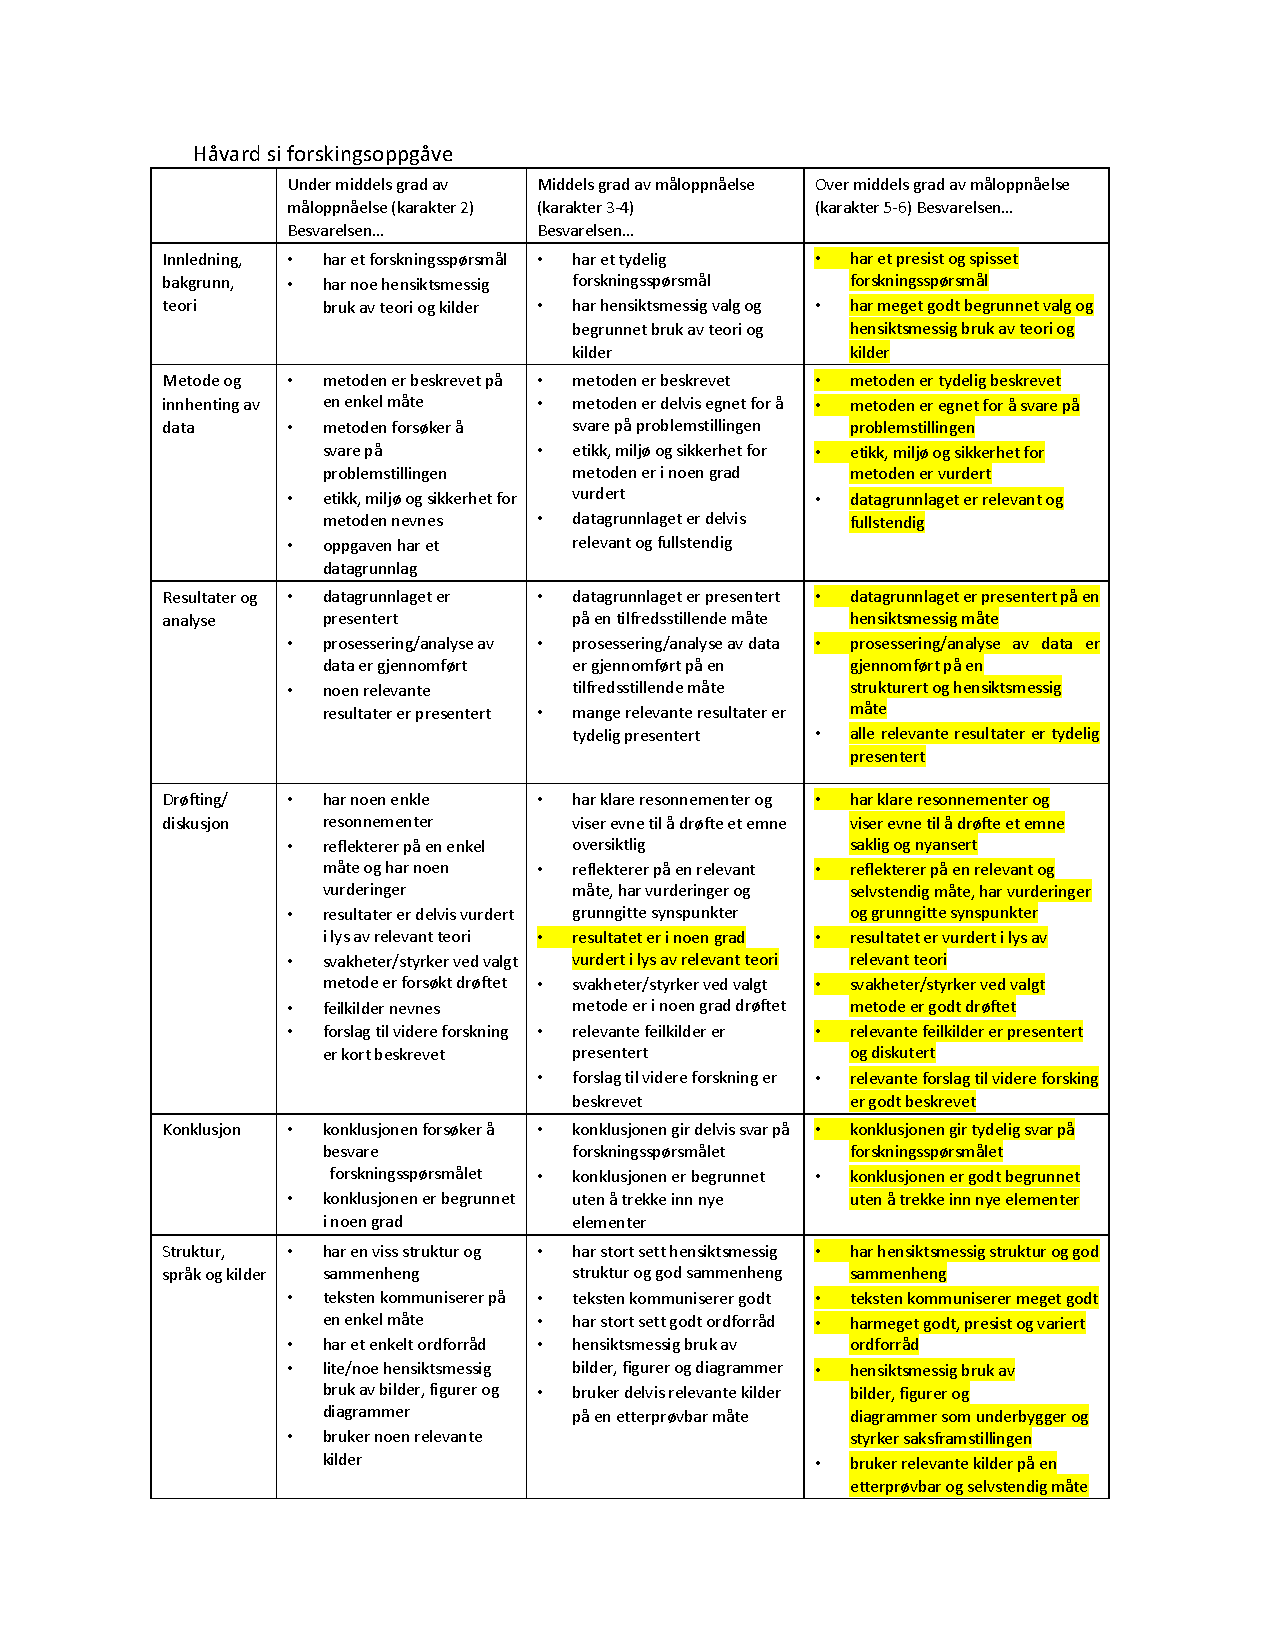
\includepdf[pages=-]{vurdering.pdf}
% Spørreundersøkelsen
\phantomsection
\addcontentsline{toc}{subsection}{Spørreundersøkelsen}
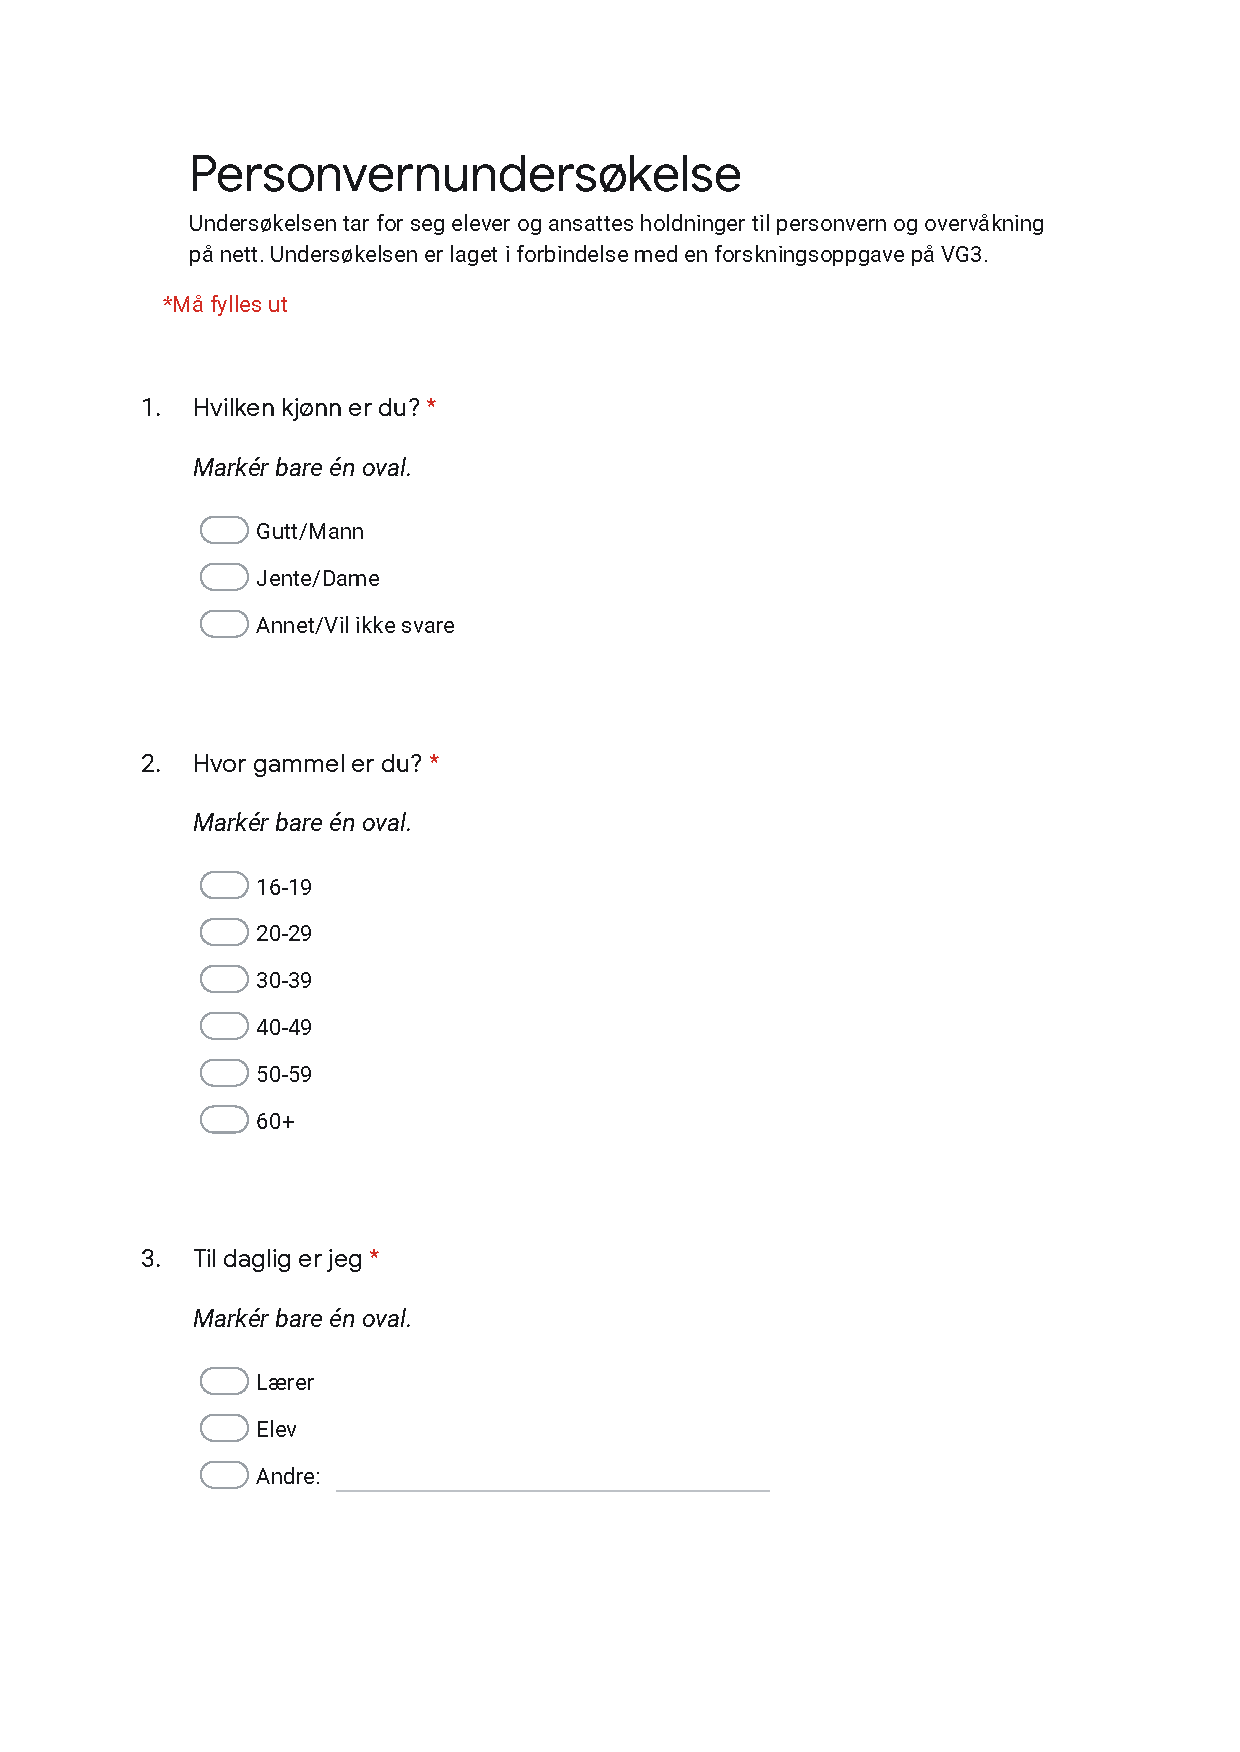
\includepdf[pages=-]{mozilla.pdf}
% Svar på spørreundersøkelsen
\phantomsection
\addcontentsline{toc}{subsection}{Svar på spørreundersøkelsen}
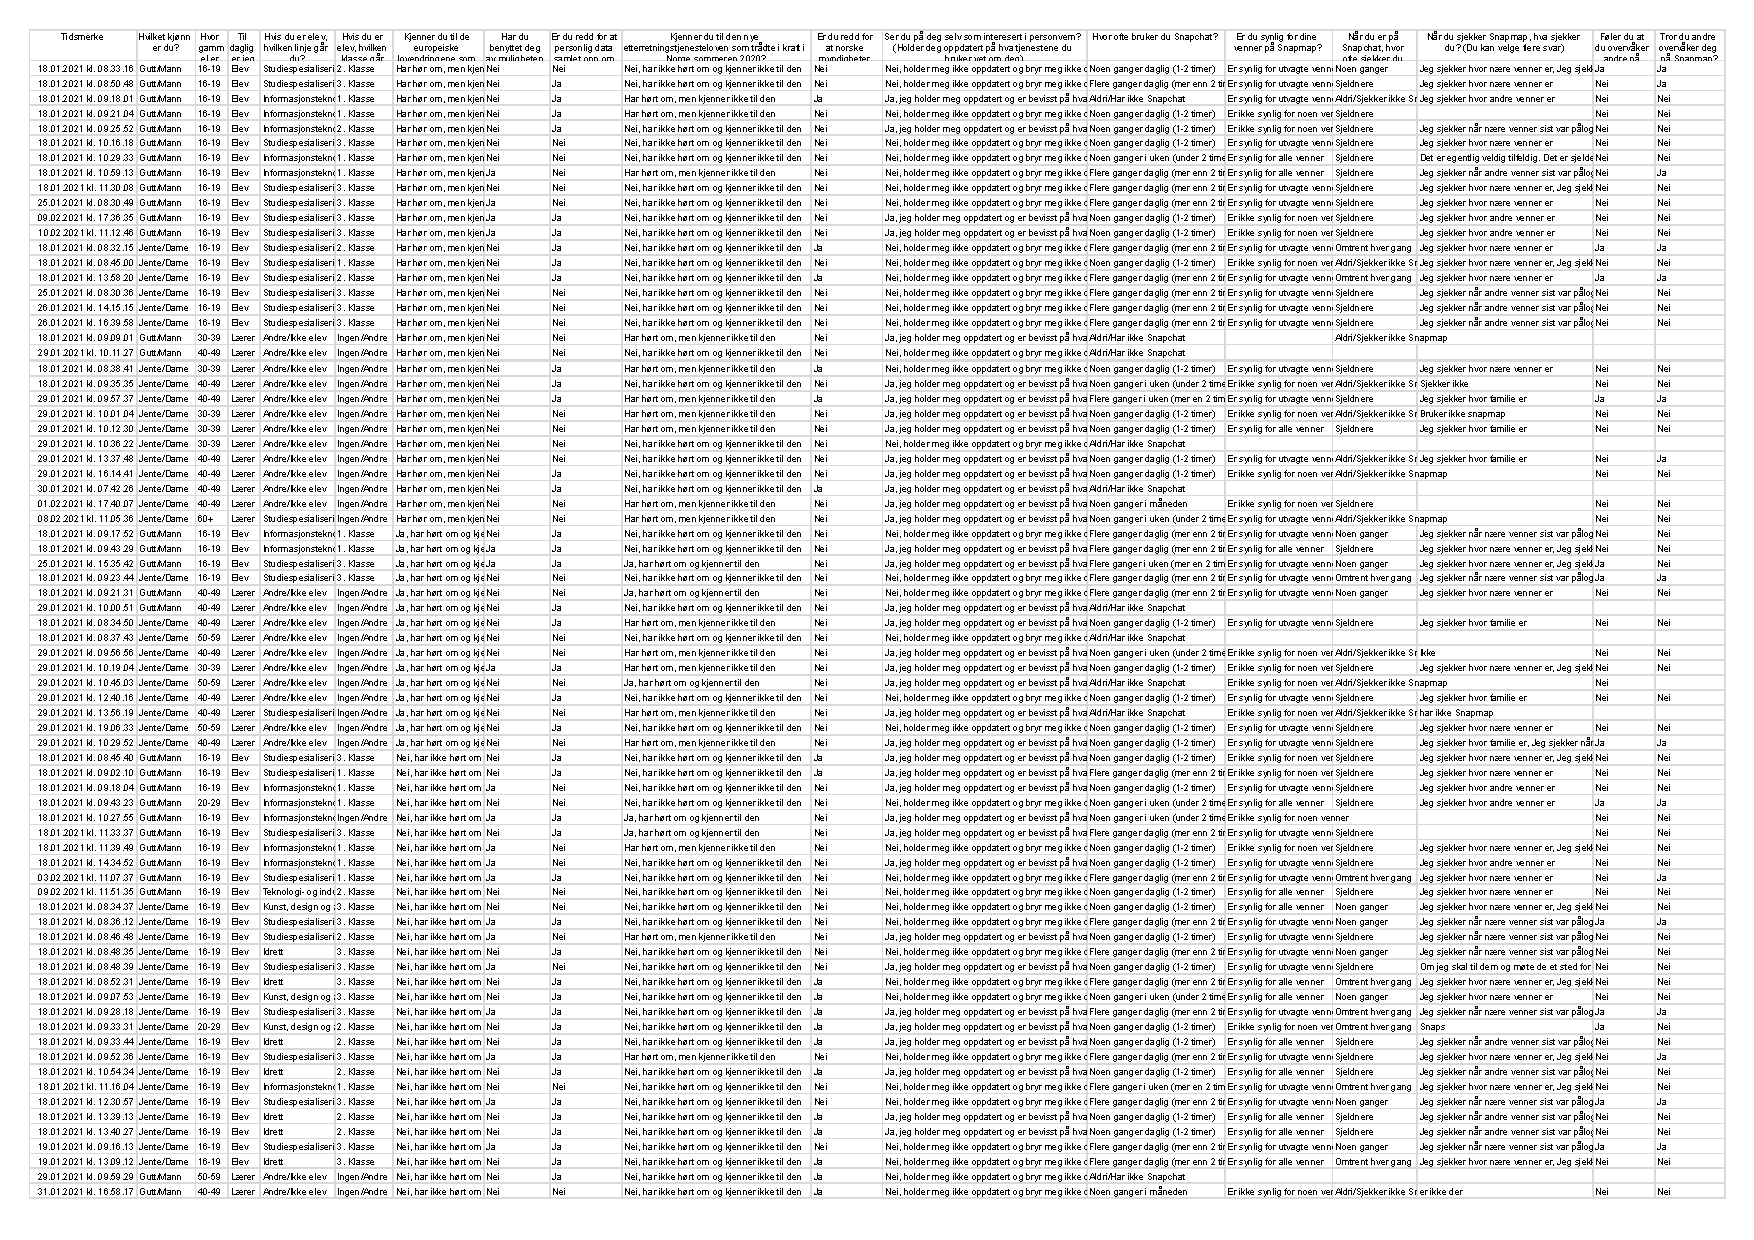
\includepdf[pages=-, angle=-90]{svar.pdf}
% Plakat til spørreundersøkelsen
\phantomsection
\addcontentsline{toc}{subsection}{Plakat til spørreundersøkelsen}

\includepdf[pages=-]{plakat.pdf}


\end{document}
